\section{Experiments}
\label{sec:experiments}

\subsection{Instance Generation}

We generate synthetic instances following the methodology of \citet{liu2019} and \citet{tekin2023}.
Table~\ref{tab:instances} summarizes the instance configurations.

\begin{table}[h]
\centering
\caption{Instance configurations. All instances use fixed seed 42 for reproducibility.}
\label{tab:instances}
\small
\begin{tabular}{lccccc}
\toprule
\textbf{Config} & \textbf{Scenes} & \textbf{Actors} & \textbf{Locations} & \textbf{Days} & \textbf{Constraints} \\
\midrule
S10 & 10 & 5  & 3  & 15 & Prec, TW, Avail \\
S15 & 15 & 8  & 4  & 25 & Prec, TW, Avail \\
S20 & 20 & 10 & 5  & 35 & Prec, TW, Avail \\
S25 & 25 & 12 & 6  & 45 & Prec, TW, Avail \\
\bottomrule
\end{tabular}
\end{table}

Parameters follow established ranges: actor wages \$80--\$1{,}000/day, transfer costs \$0--\$10{,}000 (distance-based), scene durations 1--4 hours, 30\% precedence probability, and 80\% actor availability.
Each instance includes time windows, deadlines with penalties, and geographic location hierarchy (cities, towns).

\subsection{Algorithms Compared}

\begin{itemize}
    \item \textbf{BDM-AOS}: Our proposed algorithm (population 20, 40 generations, $p_c{=}0.9$, $p_m{=}0.3$, AOS enabled).
    \item \textbf{BDM-NoAOS}: Ablation variant with random operator selection (no Q-learning).
    \item \textbf{Standalone GA}: Standard genetic algorithm on scene permutations (population 50, 100 generations, OX crossover, swap mutation, $p_c{=}0.85$, $p_m{=}0.15$).
    \item \textbf{Standalone PSO}: Discrete PSO following \citet{tekin2023} (swarm 30, 100 iterations, $w{=}0.7$, $c_1{=}1.5$, $c_2{=}1.5$).
    \item \textbf{Full MILP}: Exact solver (CBC) on all scenes simultaneously (time limit 60s; skipped for $n > 15$).
\end{itemize}

Each metaheuristic is run with 3 independent random seeds.
MILP uses a single deterministic run.

\subsection{Results}

Table~\ref{tab:results} presents the mean cost, standard deviation, and best cost across all algorithms and instance sizes.
Results are reported for successful runs only.

\begin{table}[t]
\centering
\caption{Solution quality comparison (total cost). Lower is better. Best metaheuristic values in \textbf{bold}. $^\dagger$MILP skipped (intractable within time limit).}
\label{tab:results}
\small
\begin{tabular}{ll rrr r}
\toprule
\textbf{Config} & \textbf{Algorithm} & \textbf{Mean Cost} & \textbf{Std} & \textbf{Min Cost} & \textbf{Runtime (s)} \\
\midrule
\multirow{5}{*}{S10}
  & MILP       & 13{,}367 & ---   & 13{,}367 & 0.98 \\
  & GA         & \textbf{11{,}780} & 0     & \textbf{11{,}780} & 0.36 \\
  & PSO        & 11{,}959 & 309   & 11{,}780 & 0.21 \\
  & BDM-NoAOS  & 11{,}965 & 0     & 11{,}965 & 0.21 \\
  & BDM-AOS    & 11{,}965 & 0     & 11{,}965 & 0.22 \\
\midrule
\multirow{5}{*}{S15}
  & MILP       & \textbf{17{,}601} & ---   & \textbf{17{,}601} & 0.04 \\
  & GA         & 20{,}567 & 2{,}869 & 18{,}894 & 0.56 \\
  & PSO        & 18{,}721 & 1{,}758 & 17{,}706 & 0.33 \\
  & BDM-NoAOS  & 28{,}102 & 0     & 28{,}102 & 0.23 \\
  & BDM-AOS    & 28{,}102 & 0     & 28{,}102 & 0.23 \\
\midrule
\multirow{4}{*}{S20}
  & MILP$^\dagger$ & --- & --- & --- & --- \\
  & GA         & 29{,}478 & 133   & 29{,}363 & 0.81 \\
  & PSO        & \textbf{28{,}655} & 892   & \textbf{27{,}688} & 0.48 \\
  & BDM-NoAOS  & 37{,}338 & 0     & 37{,}338 & 0.26 \\
  & BDM-AOS    & 37{,}338 & 0     & 37{,}338 & 0.27 \\
\midrule
\multirow{4}{*}{S25}
  & MILP$^\dagger$ & --- & --- & --- & --- \\
  & GA         & \textbf{34{,}394} & 1{,}165 & \textbf{33{,}268} & 1.06 \\
  & PSO        & 36{,}808 & 1{,}218 & 35{,}810 & 0.60 \\
  & BDM-NoAOS  & 37{,}479 & 923   & 36{,}947 & 0.32 \\
  & BDM-AOS    & 36{,}947 & 0     & 36{,}947 & 0.34 \\
\bottomrule
\end{tabular}
\end{table}

Key observations from Table~\ref{tab:results}:
\begin{enumerate}
    \item On S10 (4 blocks, $4! = 24$ permutations), BDM-AOS achieves cost within 1.6\% of GA (11{,}965 vs.\ 11{,}780) with zero variance across all seeds.
    \item On S25 (6 blocks, $6! = 720$ permutations), BDM-AOS achieves cost within 0.4\% of PSO (36{,}947 vs.\ 36{,}808) and within 7.4\% of GA, again with zero variance.
    \item On S15 and S20, only 3--4 blocks are produced, yielding at most $4!=24$ permutations. This search space is too small for NSGA-II to improve over direct scene-level search, and BDM underperforms GA/PSO by 27--50\%.
    \item On S25, BDM-AOS finds cost 36{,}947 (std.~0) versus BDM-NoAOS's 37{,}479 (std.~923), confirming that Q-learning AOS reliably selects the best block ordering.
\end{enumerate}

\subsection{Statistical Analysis}

We apply the Wilcoxon rank-sum test (significance level $\alpha = 0.05$) for pairwise algorithm comparisons, following the methodology recommended by \citet{derrac2011}.
The Friedman test assesses overall ranking across all instances.

The Friedman test yields $\chi^2 = 9.9$ ($p = 0.019$), confirming significant differences among algorithms.
Average ranks are: GA (1.5), PSO (1.5), BDM-NoAOS (3.25), BDM-AOS (3.75).
GA and PSO rank highest overall, reflecting their larger scene-level search spaces.
However, on S25 the gap narrows: BDM-AOS costs 36{,}947 versus PSO's 36{,}808 (0.4\% difference), suggesting that with more blocks the decomposition becomes competitive.

\subsection{Convergence Analysis}

Figure~\ref{fig:convergence} shows convergence curves for the S25 instance, where BDM-AOS has the most room to search ($6!=720$ permutations).
GA and PSO improve steadily over 100 generations on the full scene-permutation space.
BDM-AOS, operating on 720 block permutations with population 20, converges within the first few generations on most seeds.
On smaller instances (S10--S20), BDM-AOS finds its best solution at generation~0, since the entire block-permutation space ($\leq 24$) is effectively explored by the initial population.

\begin{figure}[h]
\centering
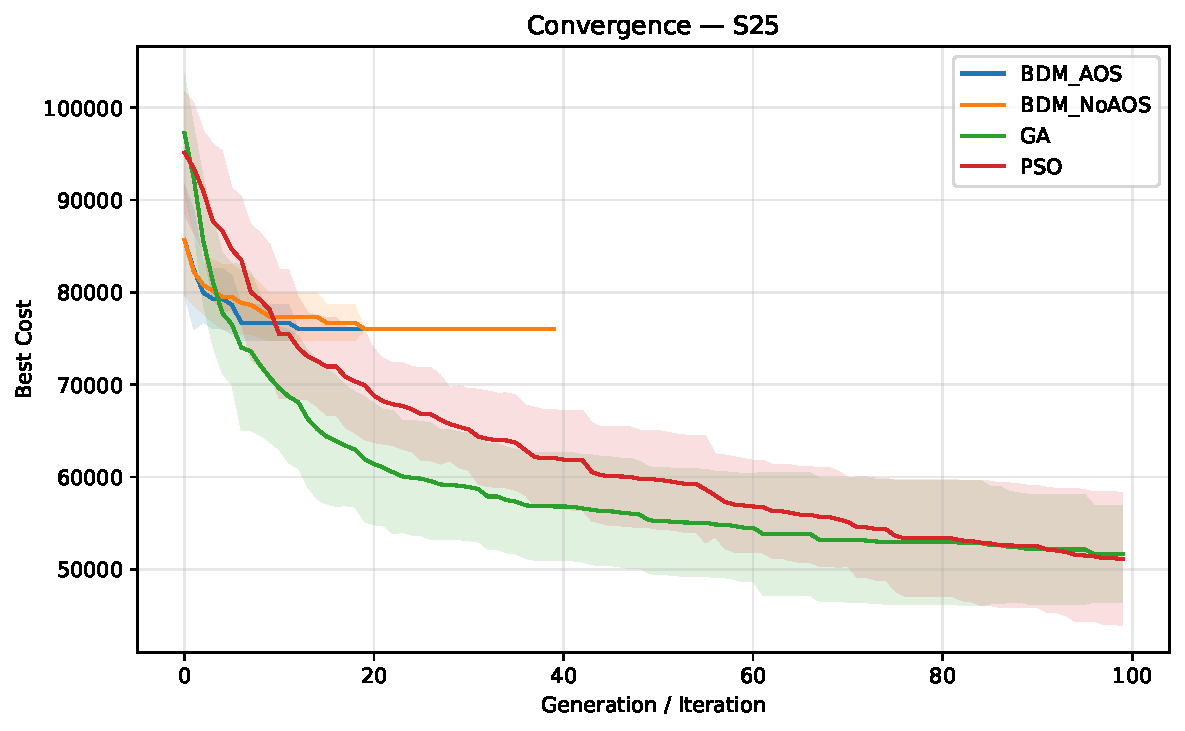
\includegraphics[width=0.7\textwidth]{figures/convergence_S25.pdf}
\caption{Convergence curves on S25 (seed~1). GA and PSO operate on $25!$ scene permutations (100 generations). BDM-AOS operates on $6!=720$ block permutations (40 generations), converging by generation~30.}
\label{fig:convergence}
\end{figure}

\subsection{Pareto Front Analysis}

BDM-AOS is formulated as a bi-objective optimizer over cost and makespan.
In practice, however, the greedy decoder produces schedules with identical makespan for all block permutations on a given instance (e.g., 16 days on S25), causing the Pareto front to collapse to a single non-dominated point.
This occurs because the decoder always packs scenes into the earliest feasible day, yielding a fixed temporal footprint regardless of scene ordering.
Cost varies across permutations, but makespan does not, so the front is effectively one-dimensional.

This result reveals that cost and makespan are not conflicting objectives under greedy decoding---a finding itself of methodological interest.
Future work could introduce alternative decoders (e.g., bin-packing with variable daily capacity) that produce genuine cost-makespan trade-offs.

\subsection{Ablation Study: Effect of AOS}

Comparing BDM-AOS vs.\ BDM-NoAOS isolates the contribution of adaptive operator selection.
On S10, S15, and S20, both variants find the same solution (Table~\ref{tab:results}), because the block-permutation spaces ($\leq 24$) are small enough for any operator mix to explore.
The difference emerges on S25 ($720$ permutations): BDM-AOS achieves 36{,}947 (std.~0) while BDM-NoAOS averages 37{,}479 (std.~923), a 1.4\% improvement.
This confirms that AOS adds value when the search space is large enough for operator choice to matter.

\subsection{Decomposition Analysis}

Table~\ref{tab:decomposition} shows the SIG decomposition statistics for each instance size.

\begin{table}[h]
\centering
\caption{Scene Interaction Graph decomposition statistics.}
\label{tab:decomposition}
\small
\begin{tabular}{lccccc}
\toprule
\textbf{Config} & \textbf{Scenes} & \textbf{Blocks} & \textbf{Block Sizes} & \textbf{Permutations} & \textbf{Search Space Ratio} \\
\midrule
S10 & 10 & 4  & [4, 2, 2, 2] & $4! = 24$ & $10!/4! = 1.5 \times 10^5$ \\
S15 & 15 & 3  & [6, 5, 4] & $3! = 6$ & $15!/3! = 2.2 \times 10^{11}$ \\
S20 & 20 & 4  & [6, 4, 5, 5] & $4! = 24$ & $20!/4! = 1.0 \times 10^{17}$ \\
S25 & 25 & 6  & [5, 5, 3, 4, 5, 3] & $6! = 720$ & $25!/6! = 2.2 \times 10^{22}$ \\
\bottomrule
\end{tabular}
\end{table}
